\documentclass{article}
\usepackage[utf8]{inputenc}
\usepackage{graphicx}
\usepackage[colorlinks]{hyperref}
\usepackage{amsmath}
\usepackage{amssymb}
\graphicspath{ {images/} }

\author{Daniel Monjas Miguélez}

\title{Apuntes de Arquitectura de Sistemas}

\begin{document}
\maketitle

\newpage

\tableofcontents

\newpage

\section{Tema 1: Soporte Hardware}
\subsection{Motivación}
\begin{figure}[h]
\centering
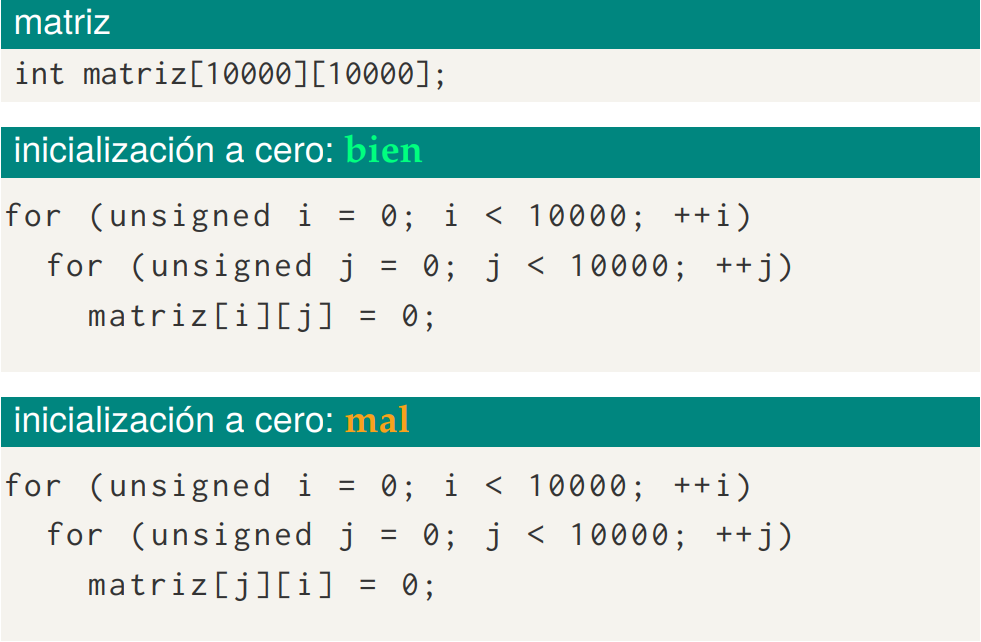
\includegraphics[scale=0.8,width=\textwidth]{gestion_memoria.png}
\end{figure}
\newpage

Para una matriz de tamaño $10000\times 10000$:
\begin{figure}[h]
\centering
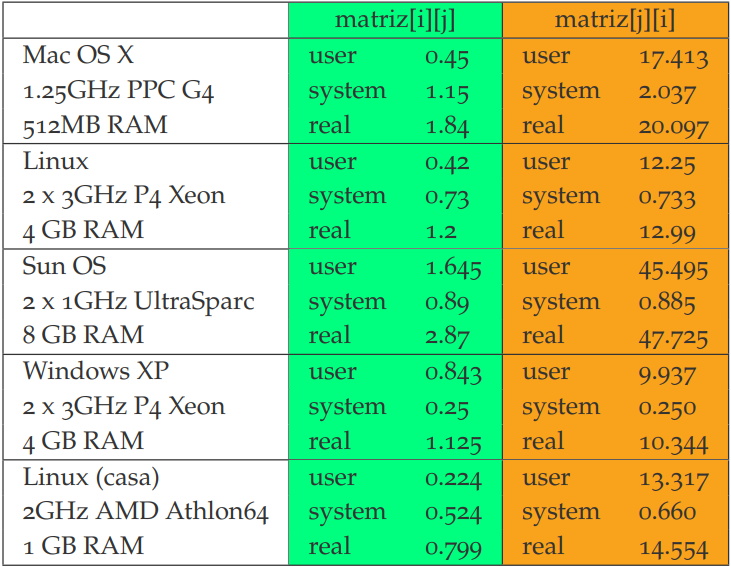
\includegraphics[scale=0.8,width=\textwidth]{time.png}
\end{figure}

La causa de este fenómeno es la forma en que C gestiona la memoria, pues C/C++ almacenan las matrices por filas. Ejemplo: $int\:\:m[4][4]$
\begin{figure}[h]
\centering
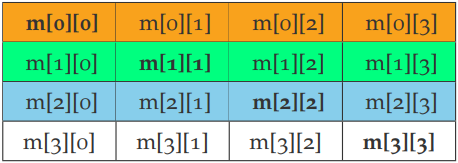
\includegraphics[scale=0.6,width=80mm]{ejemplo4x4.png}
\end{figure}

\textbf{Memoria Virtual}

Es una utilidad que permite a los programas direccionar la memoria desde un punto de vista lógico, sin importar la cantidad de memoria principal física disponible. Se concebió como método para tener múltiples trabajos de usuario residiendo en memoria principal de forma concurrente, de forma que no exista un intervalo de tiempo de espera entre la ejecución de procesos sucesivos, es decir, mientras un proceso se escribe en almacenamiento secundario y se lee el sucesor. Se introdujeron los sistemas de paginación, que permiten que los procesos se compriman en un número determinado de bloques de tamaño fijo, denominados páginas. Un programa referencia a una palabra por medio de una dirección virtual, que consiste en un número de página y un desplazamiento dentro de la página.

Todas las páginas de un proceso se mantienen en disco. Cuando un proceso está en ejecución, algunas de sus páginas se encuentran en memoria principal, y si se referencia a una página que no está en memoria principal el hardware de gestión de memoria lo detecta y permite que la página que falta se cargue (carga bajo demanda).

\subsection{Clasificación}
\subsubsection{Clasificación "práctica" de arquitecturas paralelas}
\begin{itemize}
\item Multiprocesadores de memoria compartida:
	\begin{itemize}
	\item SMT(Simultaneos Multithreading/Hyperthreading): permite a una única CPU ejecutar varios flujos de control. Esto requiere tener múltiples copias de algunos componentes hardware de la CPU, como contadores de programa y registros de archivo, mientras otras partes siguen siendo únicas como las unidades que realizan aritmética con punto flotante. Cuando un procesador tiene Hyper-Threading puede tener de 2 a 64 hebras (puede tener más, veanse procesadores de servidor), dependiendo del número de núcleos físicos del mismo.
	
	\begin{figure}[h]
	\centering
	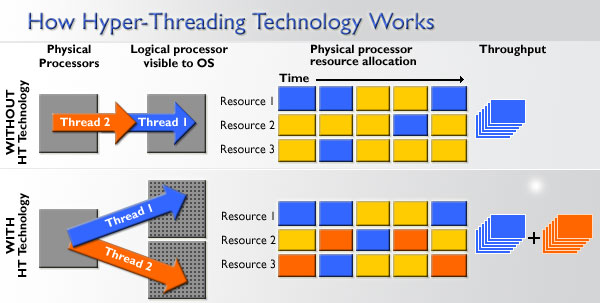
\includegraphics[scale=1,width=\textwidth]{Hyperthreading.jpg}
	\end{figure}
	
	\item SMP(Symmetric Multi-Processing): el núcleo puede ejecutar en cualquier procesador, y normalmente cada procesador realiza su propia planificación del conjunto disponible de procesos e hilos. El núcleo puede construirse como múltiples procesos o múltiples hilos, permitiéndose la ejecución de partes del núcleo en paralelo. El enfoque SMP complica el sistema operativo, ya que debe asegurar que dos procesadores no seleccionan un mismo proceso y que no se pierde ningún proceso de la cola. Se deben emplear técnicas para resolver y sincronizar el uso de los recursos. Suelen tener entre 2 y 256 procesadores.
	
	\begin{figure}[h]
	\centering
	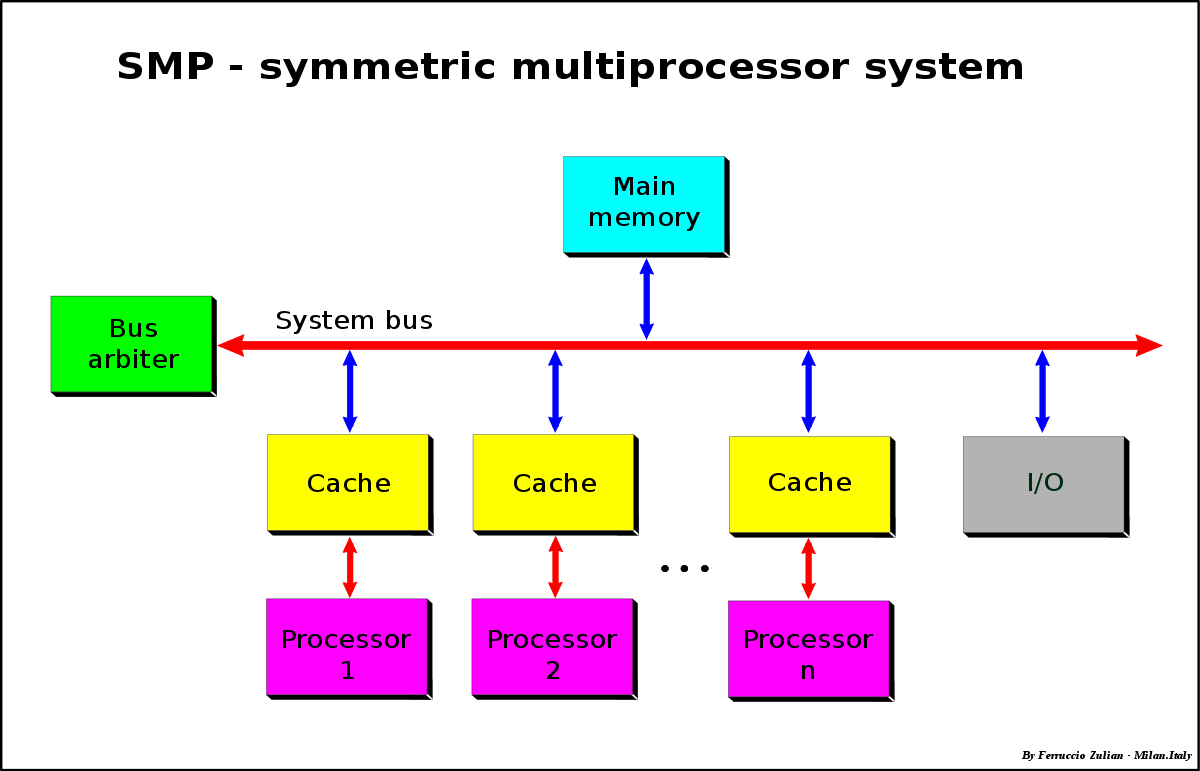
\includegraphics[scale=1,width=\textwidth]{SMP.png}
	\end{figure}
	
	\item UMA/ccNUMA (Uniforma Memory Access/Cache Coherent  UMA): Se define como la situación en la cual el acceso a cualquier RAM desde CPU toma siempre la misma cantidad de tiempo. Suele tener entre 2 y 4096 procesadores.
	
	\end{itemize}
	
\item Multiprocesadores masivamente paralelos:
	\begin{itemize}
	
	\item NUMA/ccNUMA (Non Uniform Memory Access/ Cache Coherent NUMA): A diferencia de UMA, algunas partes de la memoria pueden tomar más tiempo de acceso que otras, creando una penalización en el rendimiento. Esta penalización se puede minimizar por medio de la administración de recursos.
	
	\begin{figure}[h]
	\centering
	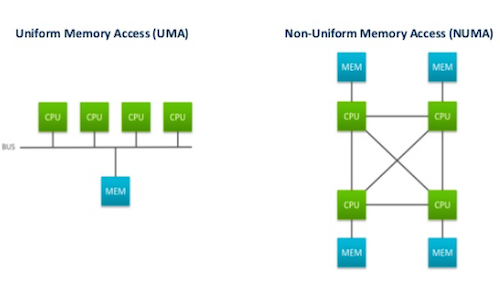
\includegraphics[scale=1,width=65mm]{umanuma.png}
	\end{figure}
	
	\item Paso de mensajes/NoRMA (No Remote Memory Access): en las arquitecturas NoRMA, el espacio de direcciones global no es único y la memoria no es globalmente accesible desde todos los procesadores. El acceso a modulos de memoria remotos es solo posible indirectamente a través del paso de mensajes por medio de la red de interconexión a otros procesadores, lo que en respuesta recibirá los datos buscados en un mensaje de respuesta.
	
	\begin{figure}[h]
	\centering
	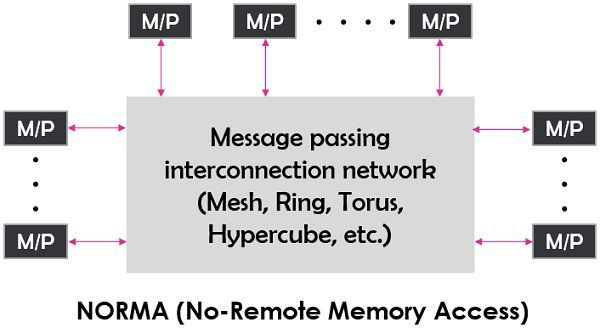
\includegraphics[scale=1,width=80mm]{NORMA.jpg}
	\end{figure}
	\end{itemize}
	
\item Cluster$\rightarrow$+10M procesadores. Al igual que los sistemas multiprocesadores, los sistemas clústes juntan múltiples CPUs para conseguir un trabajo computacional. La diferencia respecto a los sistemas multiprocesadores en que los clústers se componen de dos o más sistemas individuales unidos juntos, a los que se denominan nodos.
	\begin{itemize}
	\item GPUs
	\end{itemize}
	
	\begin{figure}[h]
	\centering
	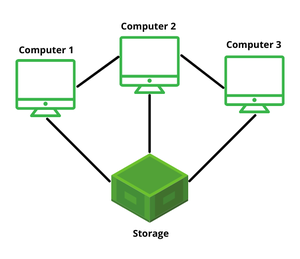
\includegraphics[scale=1,width=70mm]{cluster.png}
	\end{figure}
\end{itemize}

\subsubsection{Clasificación Arquitectura de Computadores}
\begin{itemize}
\item Sistemas monoprocesador
	\begin{itemize}
	\item Bus único
	\item Buses separados/especializados
	\end{itemize}
\item Sistemas multiprocesador
	\begin{itemize}
	\item Multiproceso simétrico (SMP)
	\item Multihebra simultánea (SMT)
	\item Multinúcleo (SMP)
	\end{itemize}
	
\item Sistemas distribuidos
\end{itemize}

\textbf{Sistema monoprocesador:} Es el modelo más simple, pues conecta todo en un bus común.
\begin{itemize}
\item Ventaja$\rightarrow$ precio.
\item Inconveniente $\rightarrow$ infrautilización de componentes por la diferencia de velocidad.
\end{itemize}

\begin{figure}[h]
\centering
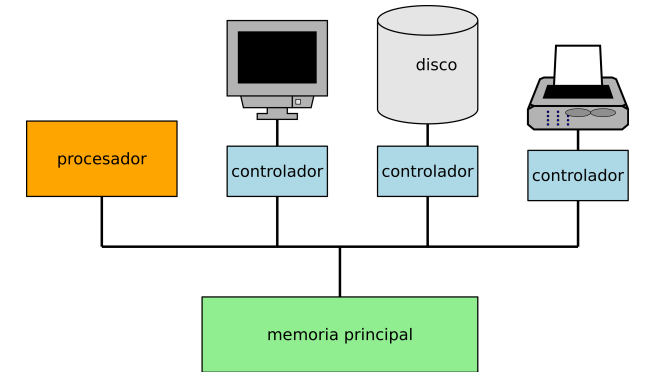
\includegraphics[scale=1,width=70mm]{monoprocesador.png}
\end{figure}

Una posible solución para la diferencia de velocidad es aislar los componentes por velocidad y conectarlos por medio de un puente

\begin{figure}[h]
\centering
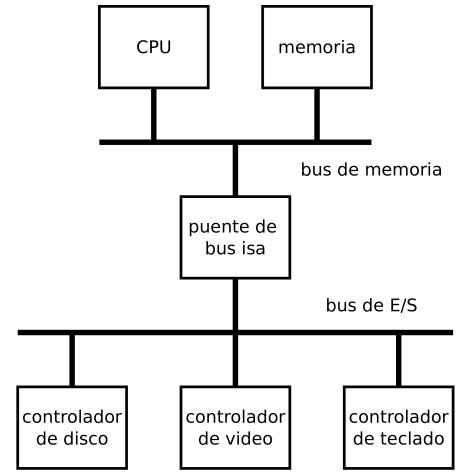
\includegraphics[scale=1,width=50mm]{solucionmonoprocesador.png}
\end{figure}
\newpage
Otra posible solución incluso mejor es separar el bus de E/S en dos buses en función de los dispositivos E/S más rápidos y más lentos, y conectar ambos buses por medio de un puente isa.

\begin{figure}[h]
\centering
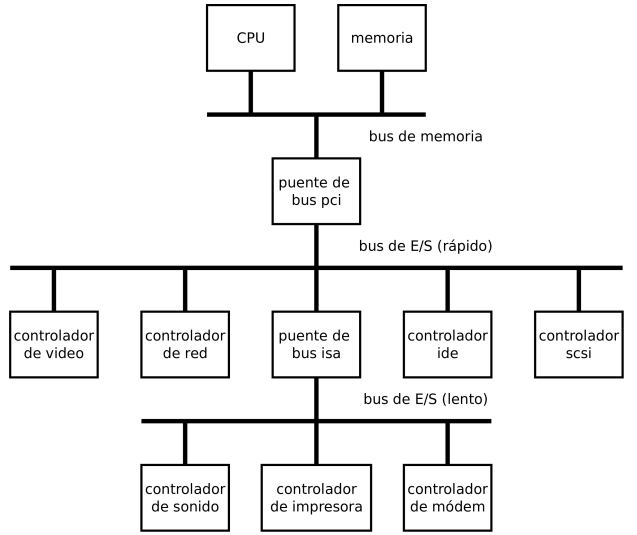
\includegraphics[scale=1,width=90mm]{sol2monoprocesador.png}
\end{figure}

\textbf{Sistema multiprocesador: multiproceso simétrico}. Lo más simple es conectar todos los elementos a un bus común.
\begin{itemize}
\item Ventaja $\rightarrow$ precio.

\item Inconveniente $\rightarrow$ se agrava la infrautilización de componentes.
\end{itemize}

\begin{figure}[h]
\centering
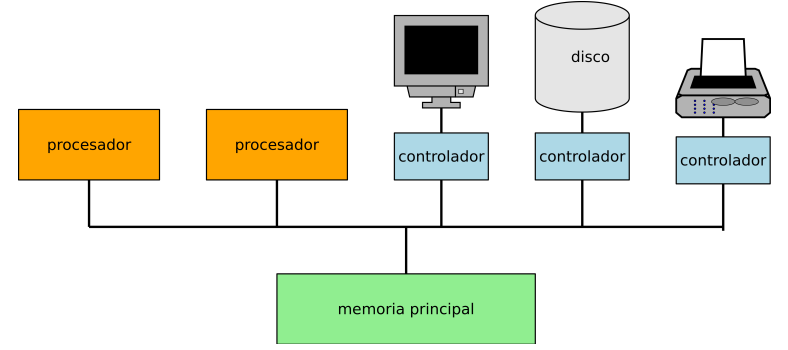
\includegraphics[scale=1,width=\textwidth]{multiprocesador.png}
\end{figure}

\newpage

\textbf{Sistemas multiprocesador: multihebra simultánea}
\begin{figure}[h]
\centering
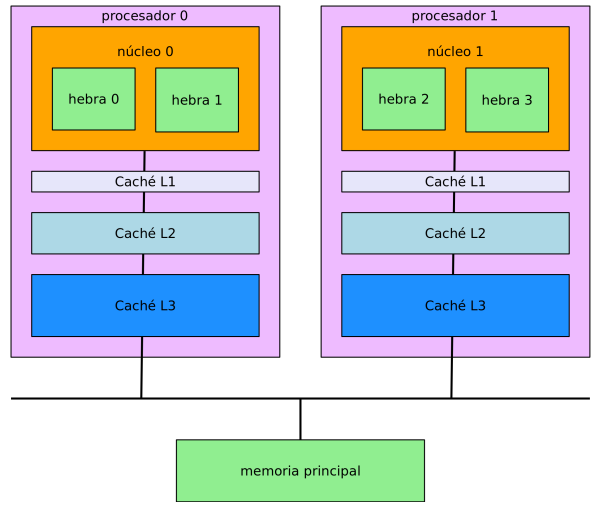
\includegraphics[scale=1,width=80mm]{multiprocesador-multihebra.png}
\end{figure}

\textbf{Sistemas multiprocesador: multiproceso simétrico}
\begin{figure}[h]
\centering
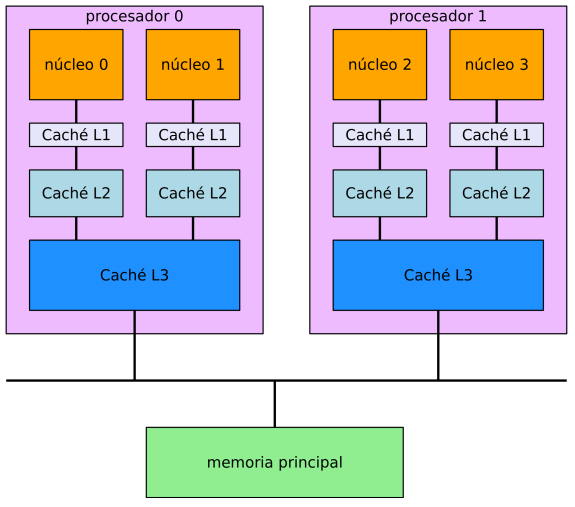
\includegraphics[scale=1,width=80mm]{multiprocesador-multihebra2.png}
\end{figure}

\newpage

\textbf{Sistemas multiprocesador actuales}
\begin{figure}[h]
\centering
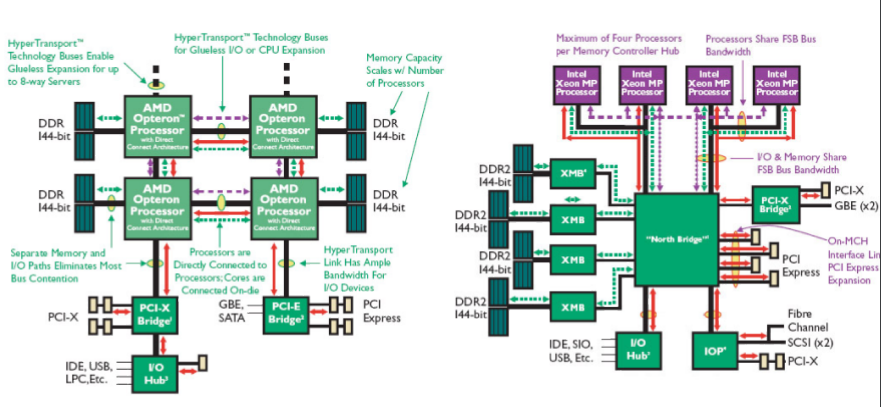
\includegraphics[scale=1,width=140mm]{multiprocesador_actual.png}
\end{figure}

\textbf{Arquitecturas de un sistema actual}
\begin{figure}[h]
\centering
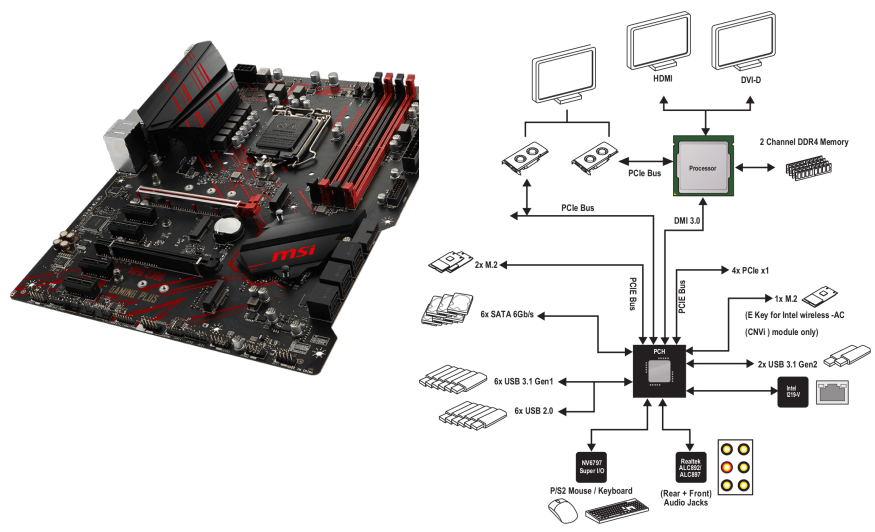
\includegraphics[scale=1,width=\textwidth]{arquitectura_actual.png}
\end{figure}


\end{document}
